%%%%%%%%%%%%%%%%%%%%%%%%%%%%%%%%%%%%%%%%%%%%%%%%%%%%%%%%%%%%%%%%%%%%%%%%%%%%%% 
\newpage
\section {Parameterization of the SINDRUM-II detector response}
\label{sec:detector_response}

%%%%%%%%%%%%%%%%%%%%%%%%%%%%%%%%%%%%%%%%%%%%%%%%%%%%%%%%%%%%%%%%%%%%%%%%%%%%%%
\subsection{Momentum resolution}

Figure ~\ref{fig:dio_1} overlays the electron momentum spectrum measured by SINDRUM-II
and the DIO spectrum on \Pb{208} calculated in \cite{Watanabe_1993} and shifted by 0.5 MeV
to account for the difference in the muon binding energies in \Pb{208} and \Au{197}. 
Both spectra are rapidly falling with momentum and have very different slopes.
The sign of the difference is easy to understand: in the case of a falling spectrum,
the finite experimental resolution smears the spectrum and reduces the observed slope. 

\vspace{0.2in}
\begin{tikzpicture}
  \node[anchor=south west,inner sep=0] at (0,0.) {
    % \node[shift={(0 cm,0.cm)},inner sep=0,rotate={90}] at (0,0) {}
    \makebox[\textwidth][c] {
      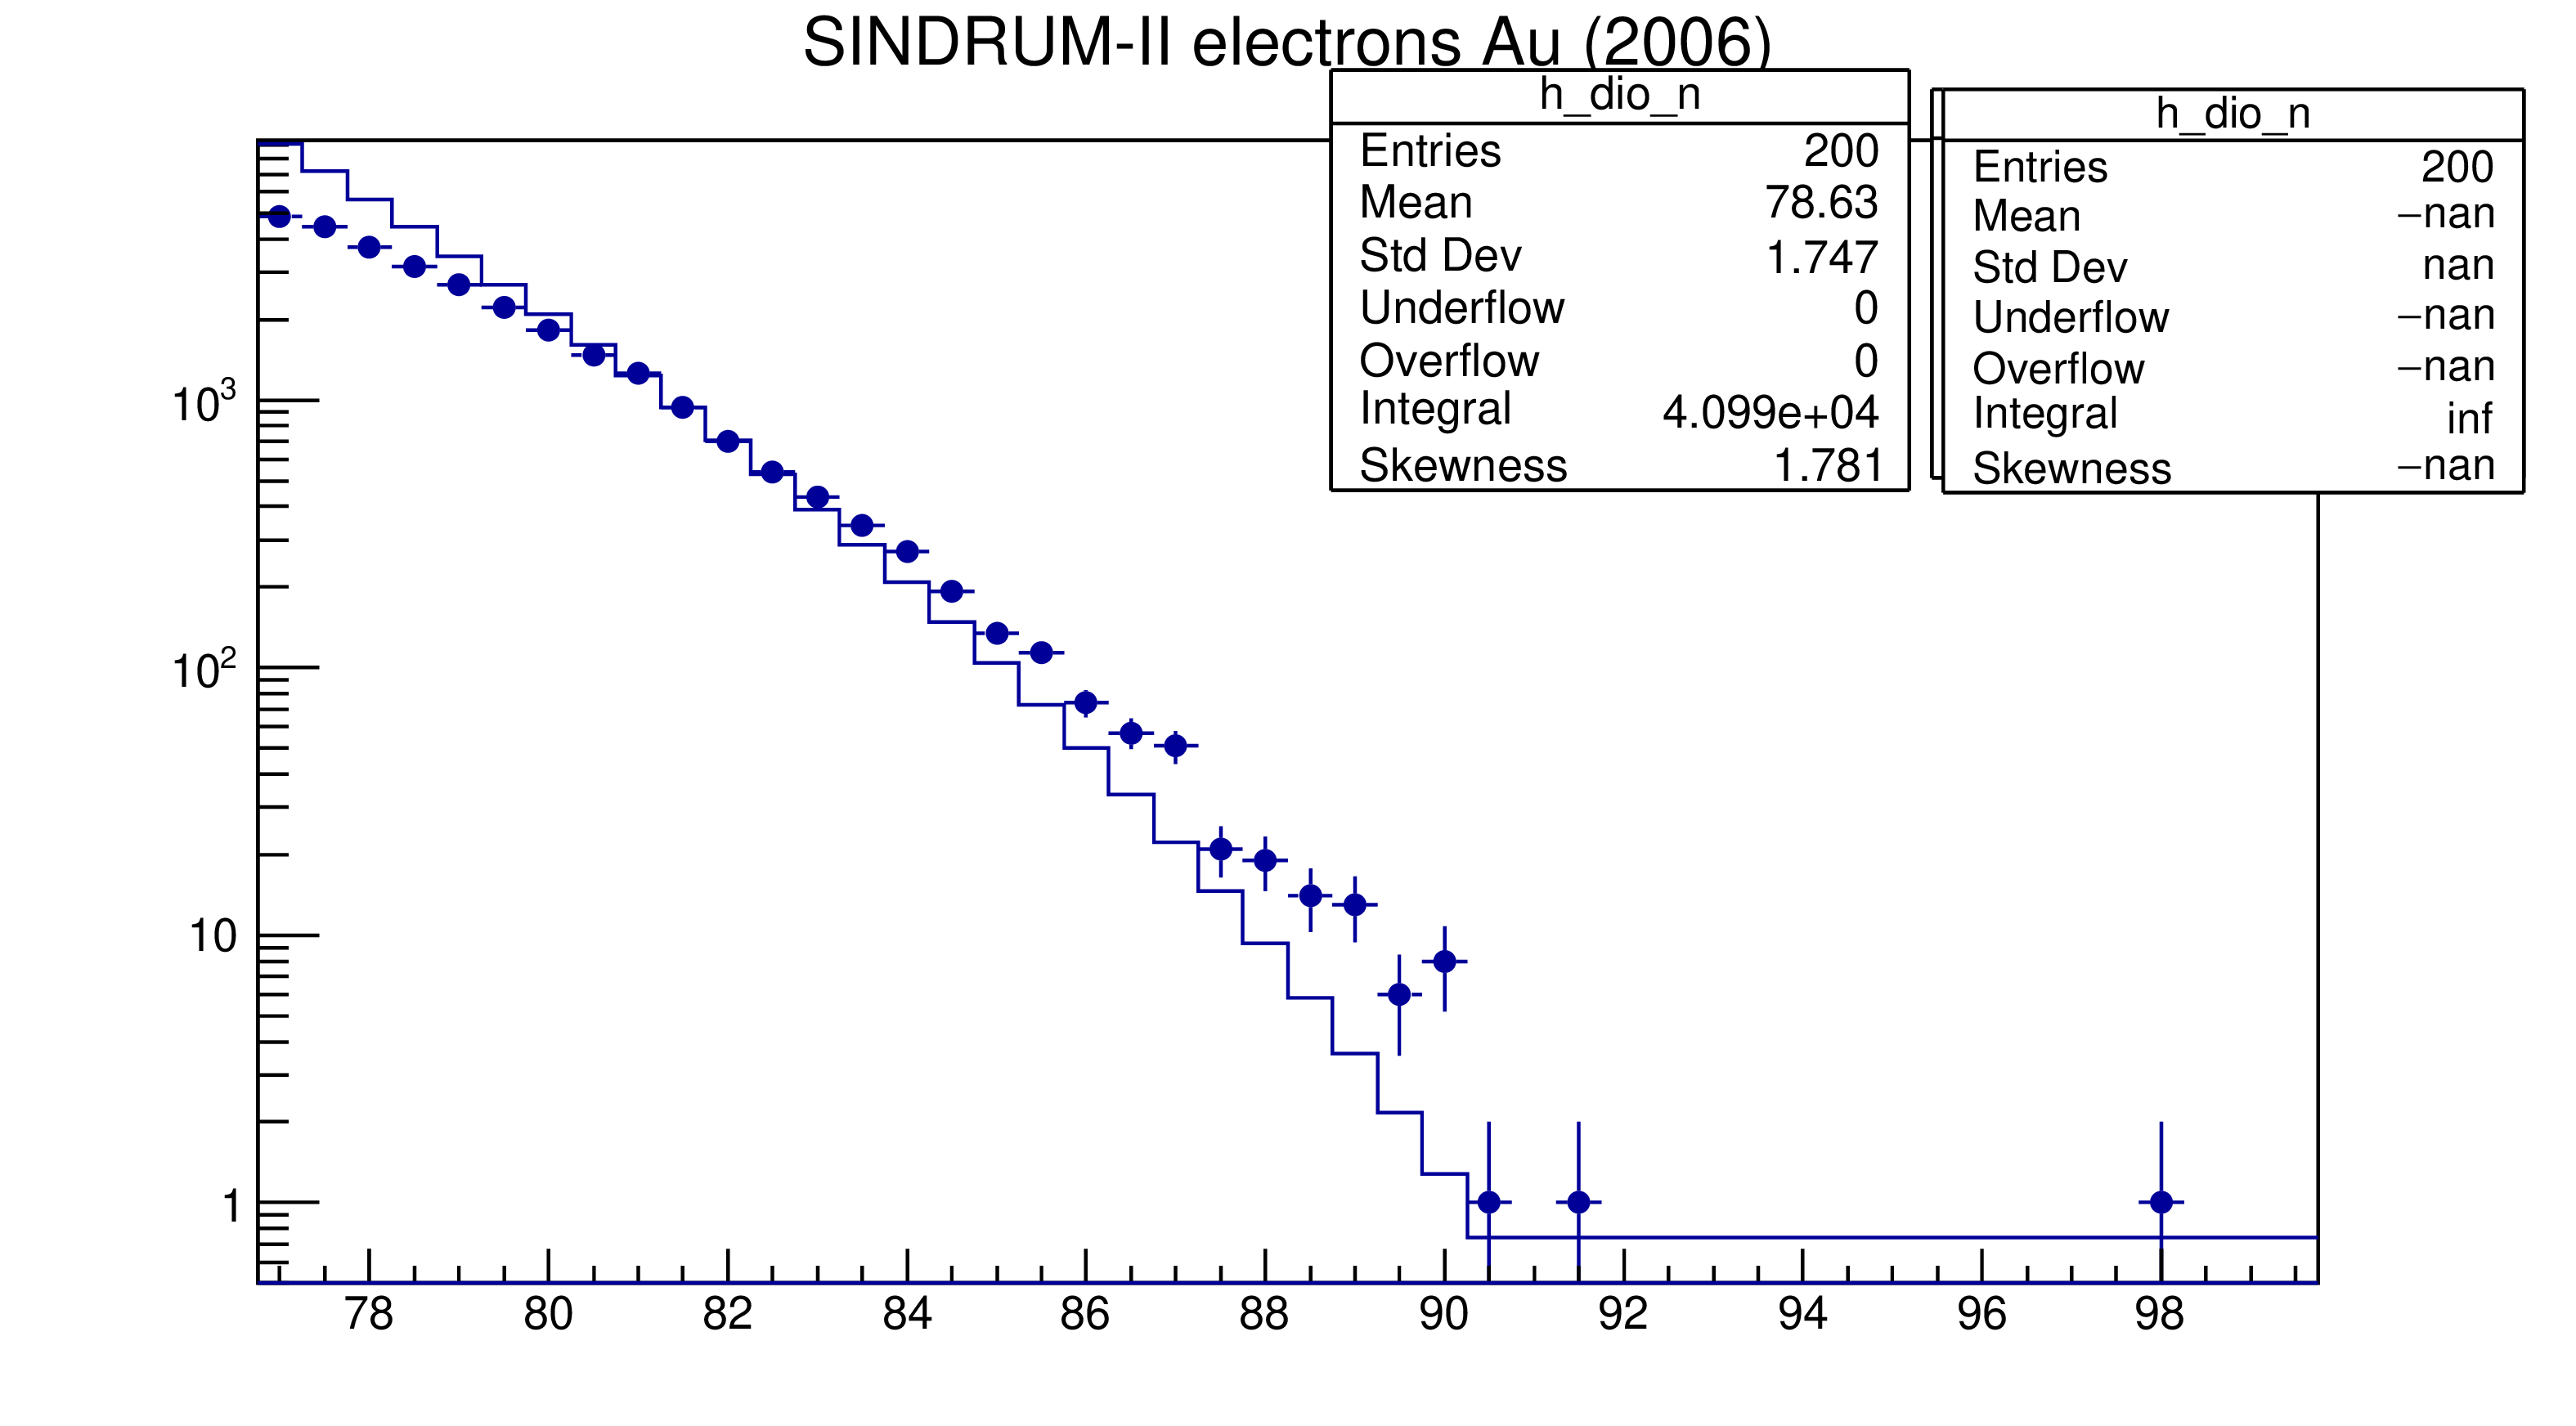
\includegraphics[width=1.0\textwidth]{figures/png/ana_step1_dio_normalized_above_80}
    }
  };
  % \node [text width=6cm, scale=0.8] at (4.5,6.4) {mu2e-18894 by Kevin Lynch and Jim Popp};
\end{tikzpicture}
\captionof{figure} {
  \label{fig:dio_1}
  SINDRUM-II electron spectrum overlaid with the DIO spectrum from \cite{Watanabe_1993}.
  The two spectra are normalized to the same area for p > 80 MeV/c.
}
\vspace{0.2in}

We make a simplifying assumption that the detector momentum response function is symmetric and
can be described by a single Gaussian. To choose the optimal value of the resolution parameter
$\sigma_P$, we vary its value in the range [1, 3.5] MeV/c, convolve the theoretical DIO spectrum
with the resolution function, and use the resulting distribution to fit the SINDRUM-II
electron spectrum. The fit has one parameter - normalization. The fit $\chi^2$ dependence
on $\sigma_P$ is shown in Figure ~\ref{fig:ana_step1_fit_sigma}.
%
The best value of the resolution parameter $\sigma_P = 2.0 \pm 0.1$ MeV/c is significantly
higher than the SINDRUM-II momentum resolution, which is about 0.5 MeV.
The difference is most likely due to the contribution of RMC electrons unaccounted for
in the fitting procedure. As one can see from Figure ~\ref{fig:sindrum_ii_2006_fig_11},
for momenta close to 90 MeV/c, the RMC contribution can not be ignored, and as the RMC spectrum
is less steep than the DIO spectrum, ignoring the RMC contribution should result in a
larger value of $\sigma_P$ returned by the fit. 

\vspace{0.2in}
\begin{tikzpicture}
  \node[anchor=south west,inner sep=0] at (0,0.) {
    % \node[shift={(0 cm,0.cm)},inner sep=0,rotate={90}] at (0,0) {}
    \makebox[\textwidth][c] {
      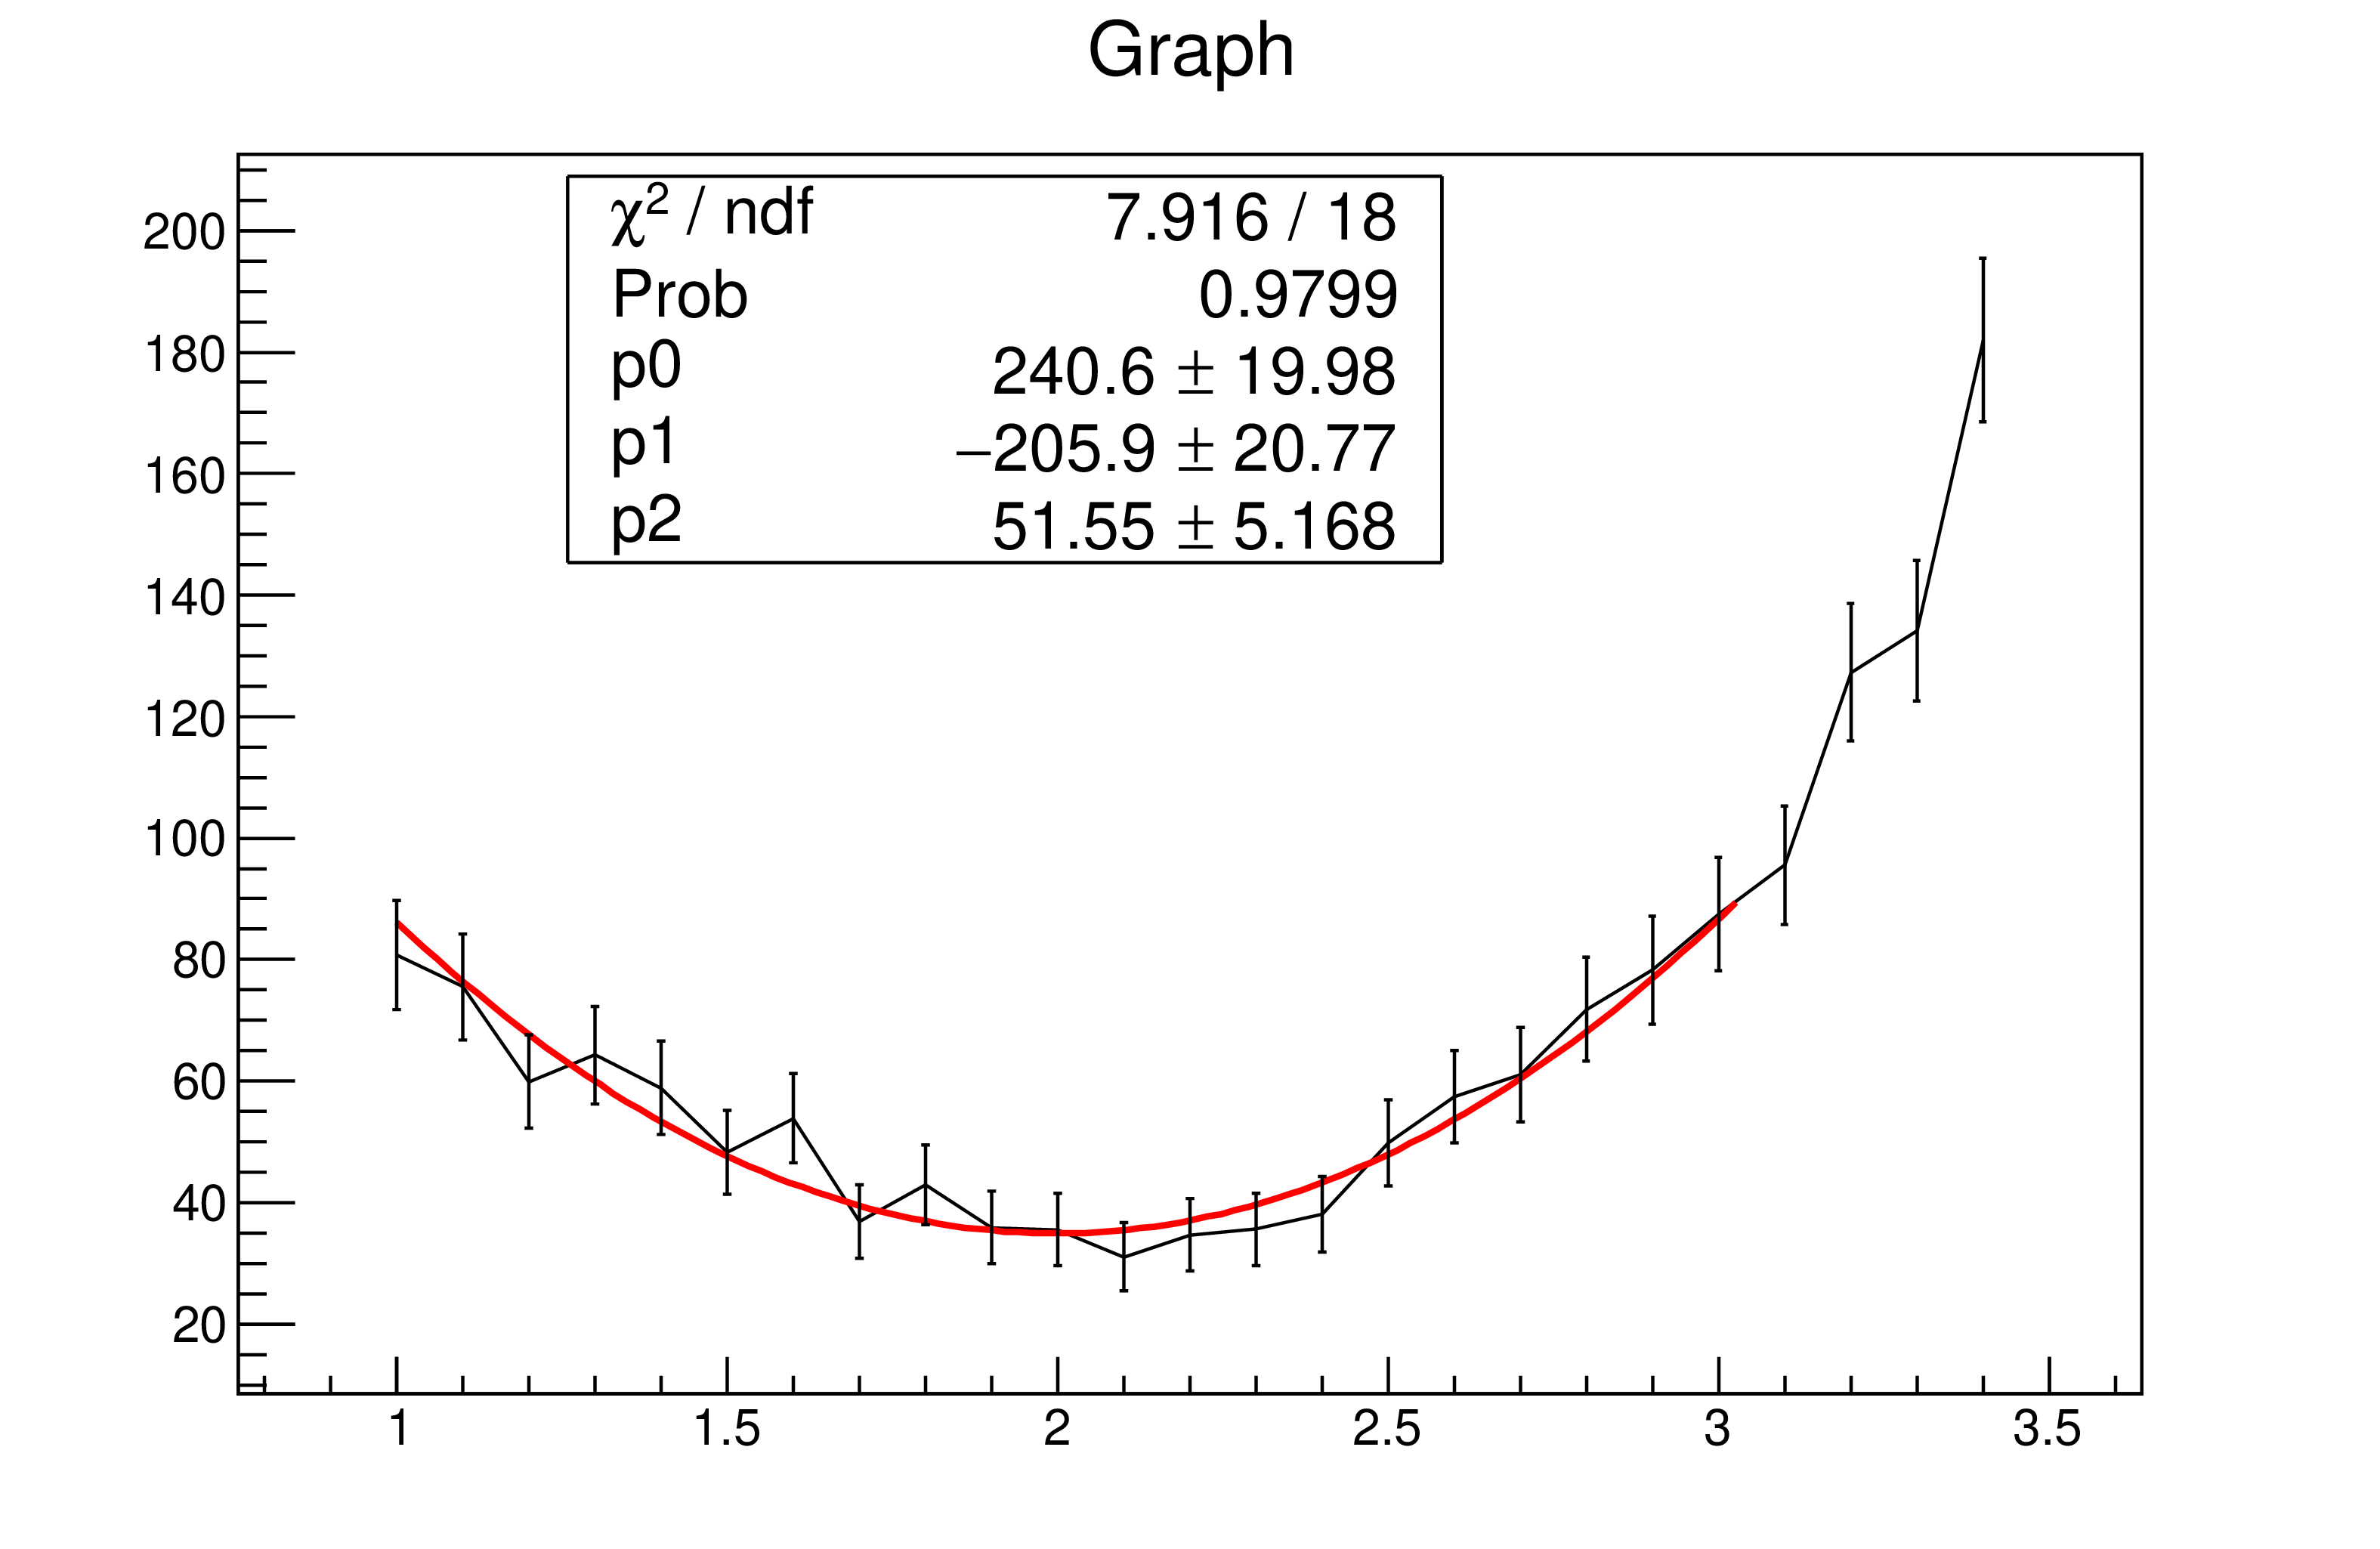
\includegraphics[width=0.9\textwidth, trim = 0 0 0 200, clip]{figures/png/ana_step1_fit_sigma}
    }
  };
  % \node [text width=6cm, scale=0.8] at (4.5,6.4) {mu2e-18894 by Kevin Lynch and Jim Popp};
\end{tikzpicture}
%
\captionof{figure} {
  \label{fig:ana_step1_fit_sigma}
  $\chi^2$ of the fit of the SINDRUM-II DIO electron spectrum with the theoretical distribution
  convolved with a Gaussian with given resolution $\sigma_P$ as a function of $\sigma_P$.
}
\vspace{0.2in}

%%%%%%%%%%%%%%%%%%%%%%%%%%%%%%%%%%%%%%%%%%%%%%%%%%%%%%%%%%%%%%%%%%%%%%%%%%%%%%
\subsection{Tracking efficiency}

To parameterize the SINDRUM-II tracking efficiency, we assume that it is flat
for momenta p> 80 MeV/c.
Normalizing the DIO spectrum convolved with a $\sigma_P = 2.0$ MeV/c Gaussian resolution
to the electron data in the region p > 80 MeV/c and dividing the data spectrum
by the resulting distribution gives the ``efficiency'' dependence on the track
momentum. The resulting dependence is shown in Figure ~\ref{fig:ana_step1_efficiency}, 
and it is fit well by a function represented by a straight line below 80 MeV/c
and a constant above 80 MeV/c.

\begin{tikzpicture}
  \node[anchor=south west,inner sep=0] at (0,0.) {
    % \node[shift={(0 cm,0.cm)},inner sep=0,rotate={90}] at (0,0) {}
    \makebox[\textwidth][c] {
      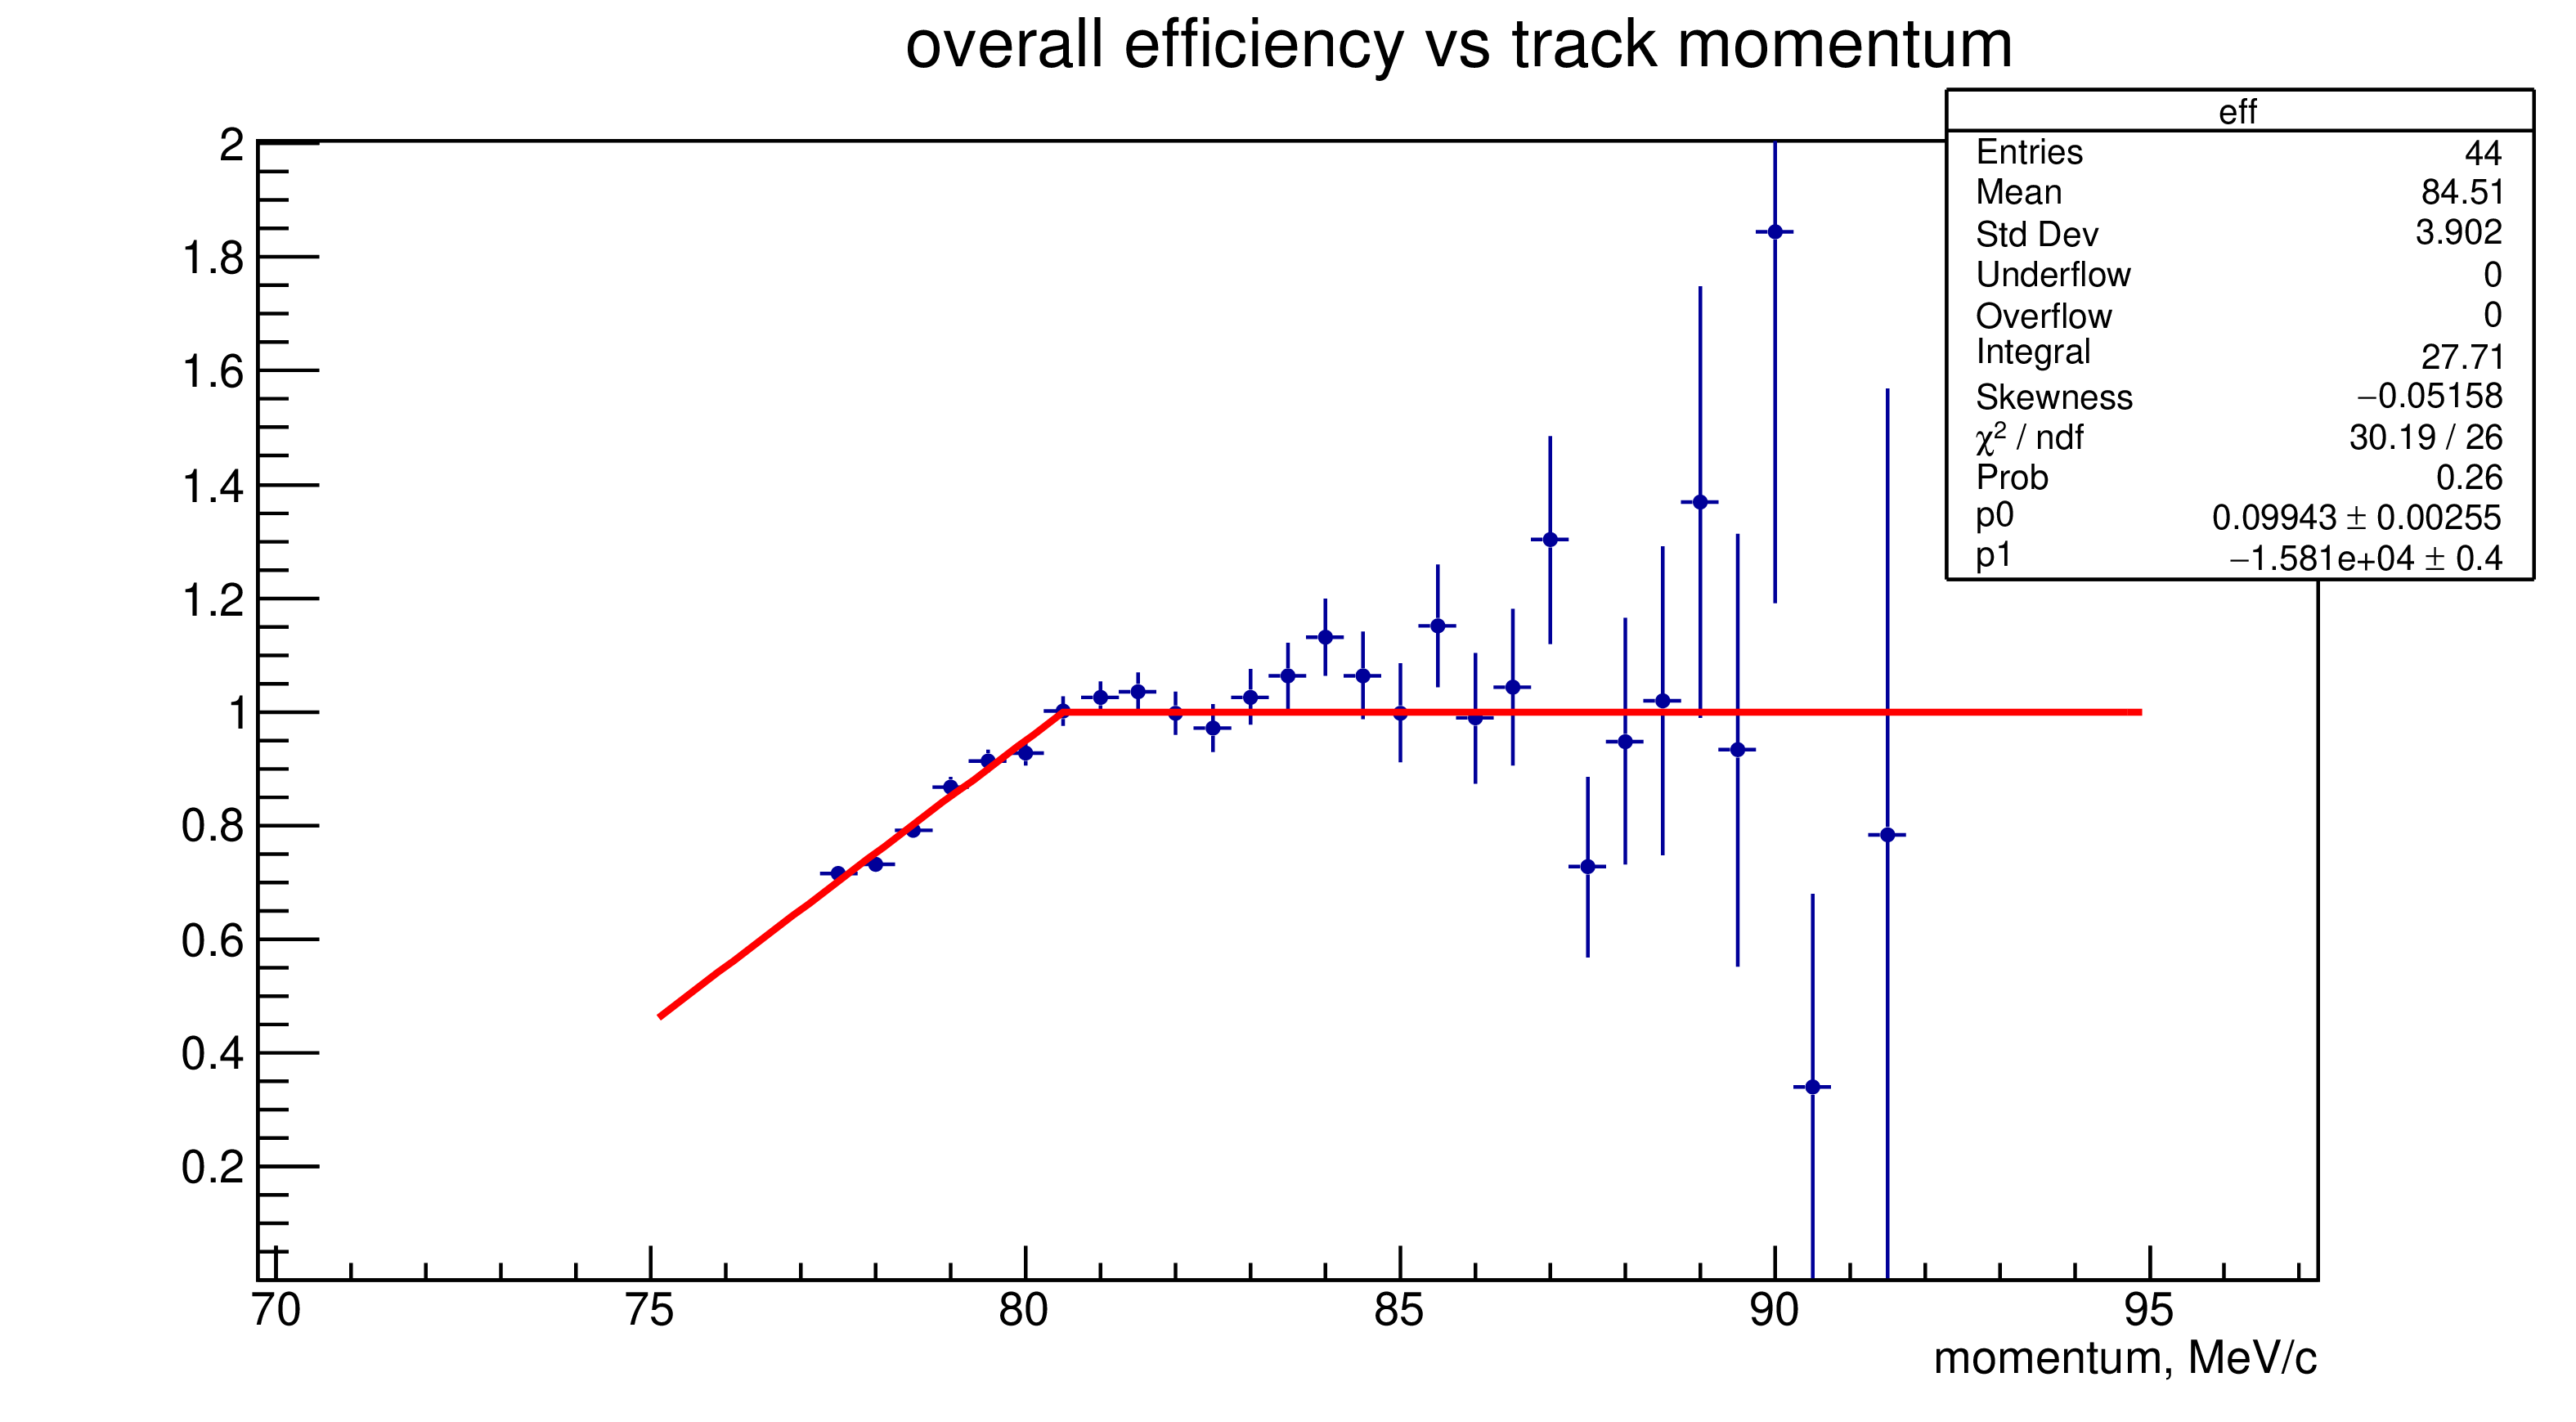
\includegraphics[width=0.9\textwidth]{figures/png/ana_step1_efficiency}
    }
  };
  % \node [text width=6cm, scale=0.8] at (4.5,6.4) {mu2e-18894 by Kevin Lynch and Jim Popp};
\end{tikzpicture}
%
\captionof{figure} {
  \label{fig:ana_step1_efficiency}
  Parameterization of the SINDRUM-II efficiency vs the track momentum.
  Definition of efficiency includes all components - trigger, reconstruction and selection.
  Overall normalization is chosen such that efficiency is equal to one for p > 80 MeV/c.
}
\vspace{0.2in}

This step concludes tuning of the detector response. Figure \ref{fig:ana_step1_best_dio_fit}
shows the description of the SINDRUM-II electron data of \cite{sindrum_ii:Bertl2006}
with the tuned response - the quality of description is surprisingly good,
better than one might expect from such a simplistic model.

\vspace{0.2in}
\begin{tikzpicture}
  \node[anchor=south west,inner sep=0] at (0,0.) {
    % \node[shift={(0 cm,0.cm)},inner sep=0,rotate={90}] at (0,0) {}
    \makebox[\textwidth][c] {
      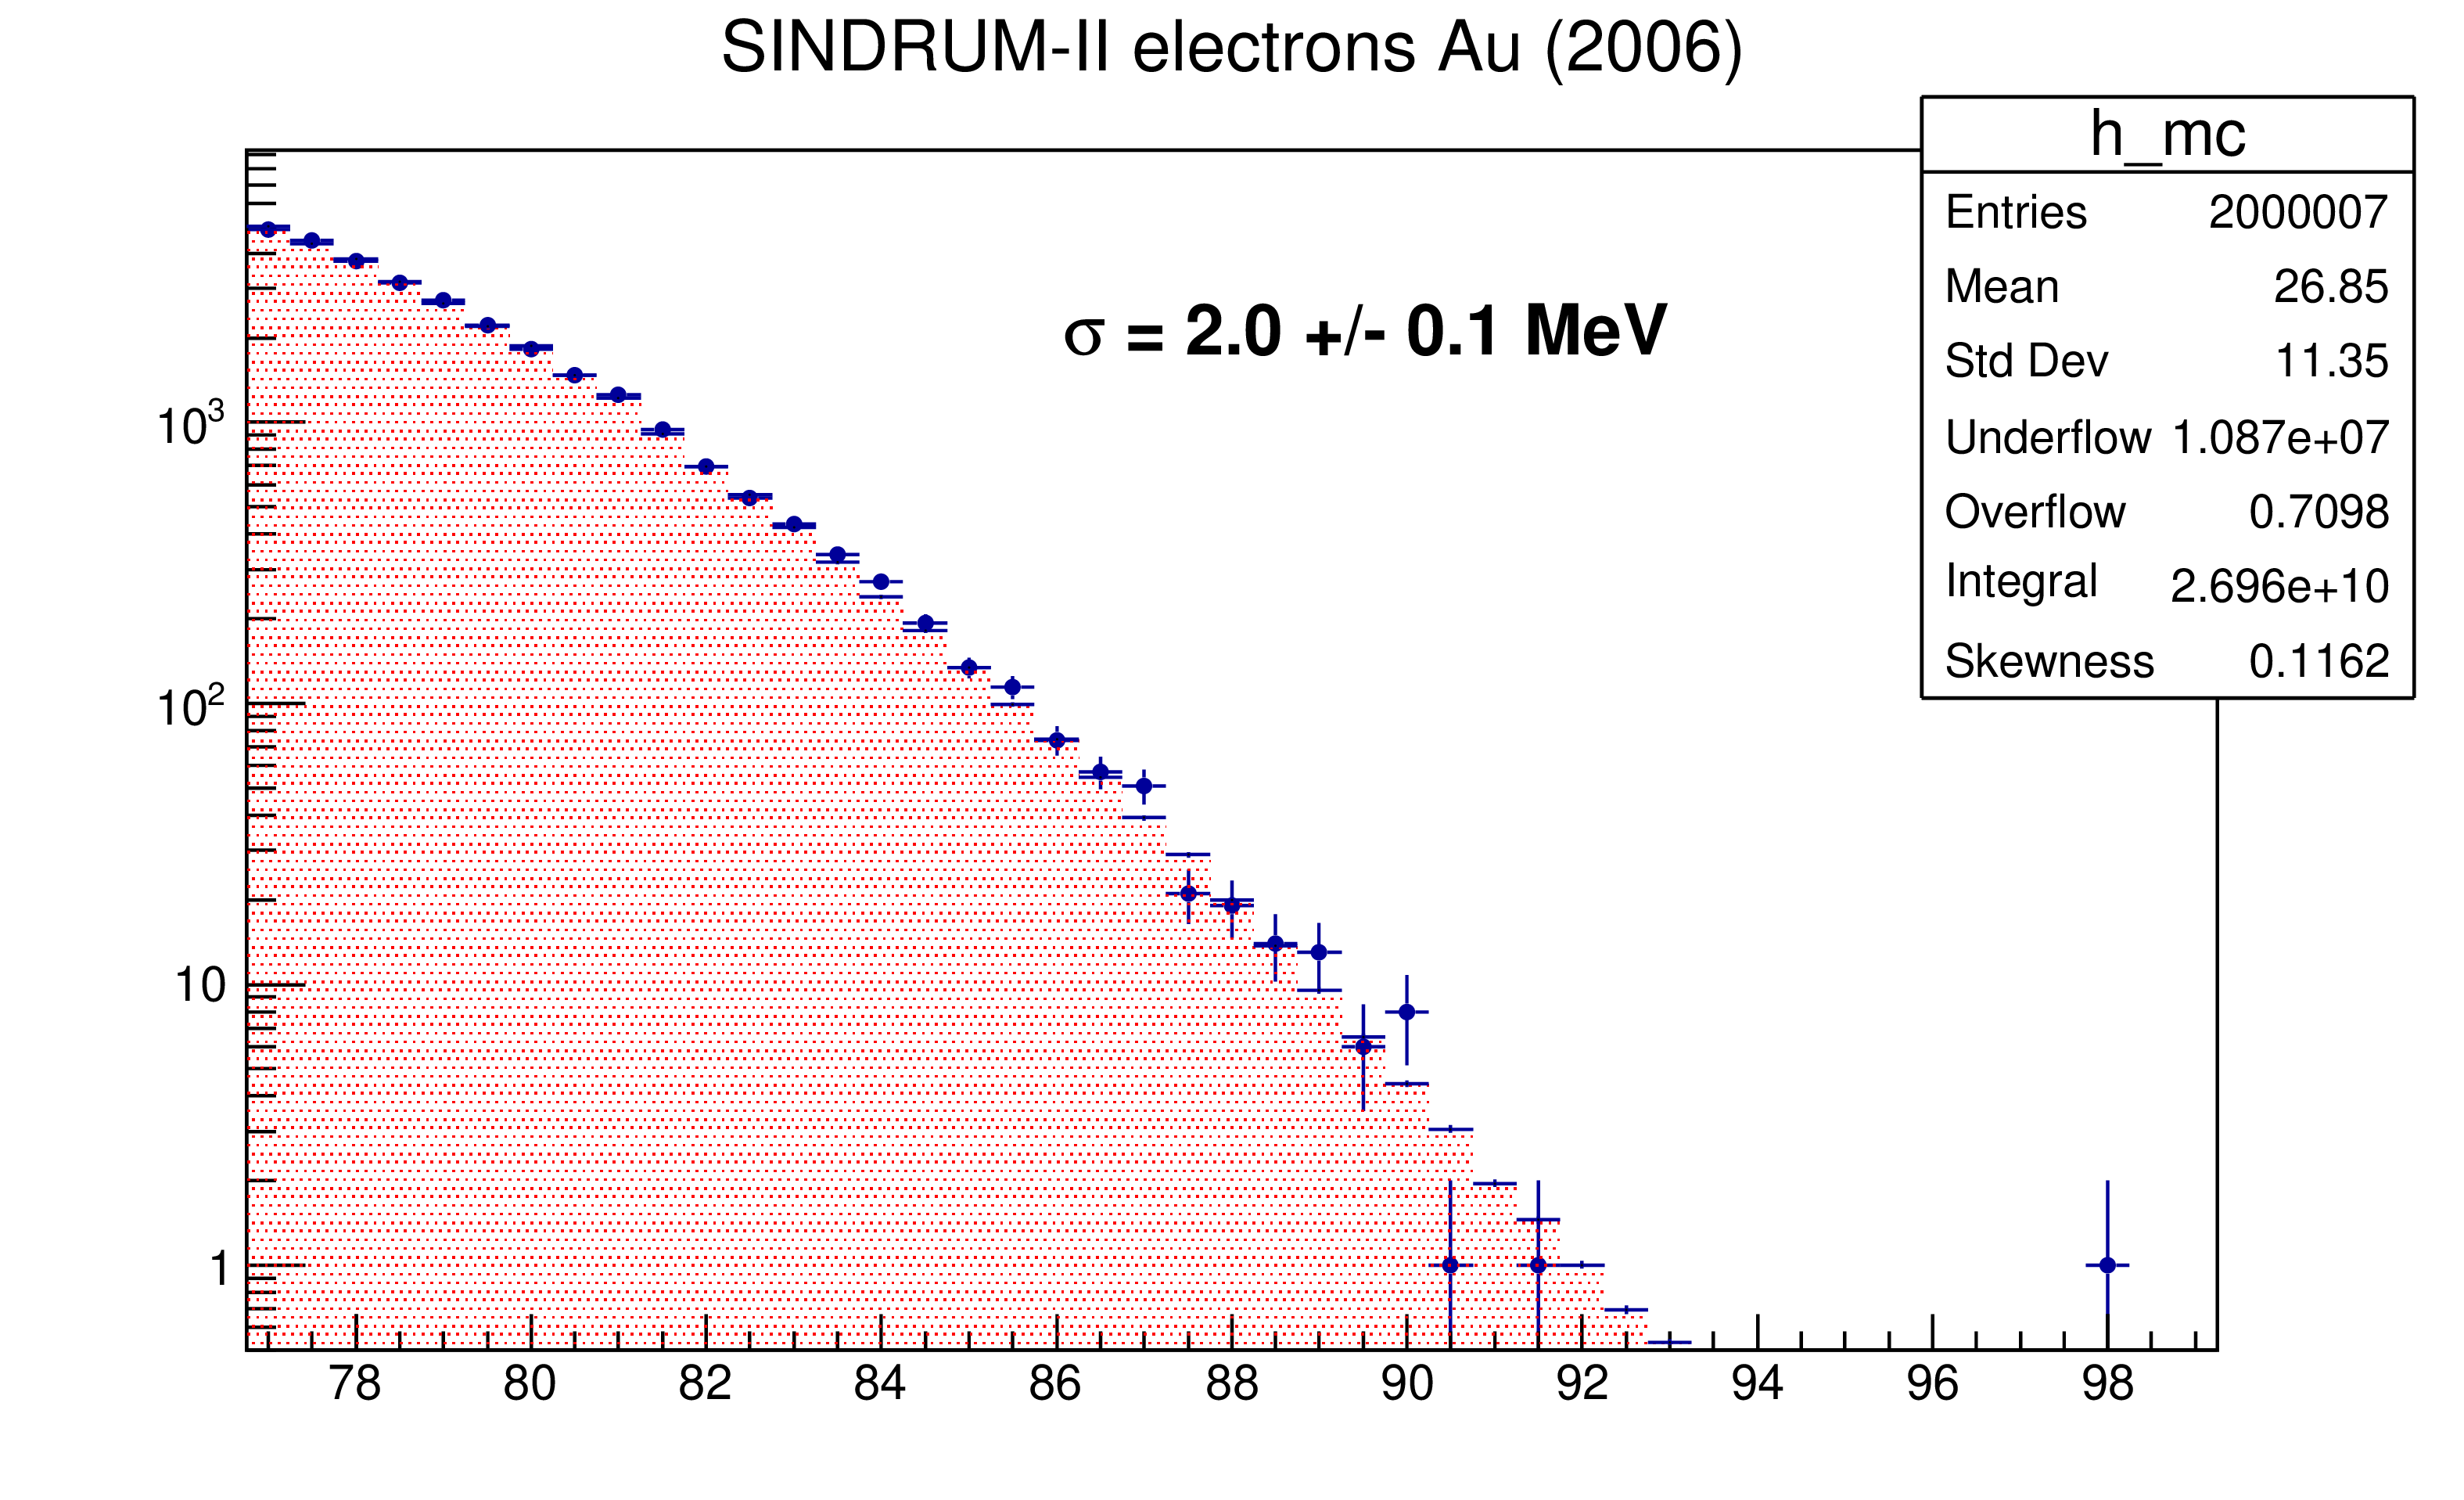
\includegraphics[width=0.99\textwidth]{figures/png/ana_step1_best_dio_fit}
    }
  };
  % \node [text width=6cm, scale=0.8] at (4.5,6.4) {mu2e-18894 by Kevin Lynch and Jim Popp};
\end{tikzpicture}
%
\captionof{figure} {
  \label{fig:ana_step1_best_dio_fit}
  Description of the electron spectrum on the Au target from \cite{sindrum_ii:Bertl2006}
  with the tuned model of the SINDRUM-II detector response.
}
